\documentclass{paper}

\usepackage[margin=1.5in]{geometry}
\usepackage{amsmath,amsthm,amssymb,hyperref,tikz,scrextend}
\usepackage[ruled,vlined]{algorithm2e}
\usepackage[most]{tcolorbox}
\usepackage{hyperref}
\hypersetup{
    colorlinks=true,
    linkcolor=blue,
    filecolor=magenta,      
    urlcolor=cyan,
}

\newcommand{\R}{\mathbf{R}}  
\newcommand{\Z}{\mathbf{Z}}
\newcommand{\N}{\mathbf{N}}
\newcommand{\Q}{\mathbf{Q}}

\newenvironment{theorem}[2][Theorem]{\begin{trivlist}
\item[\hskip \labelsep {\bfseries #1}\hskip \labelsep {\bfseries #2.}]}{\end{trivlist}}
\newenvironment{lemma}[2][Lemma]{\begin{trivlist}
\item[\hskip \labelsep {\bfseries #1}\hskip \labelsep {\bfseries #2.}]}{\end{trivlist}}
\newenvironment{claim}[2][Claim]{\begin{trivlist}
\item[\hskip \labelsep {\bfseries #1}\hskip \labelsep {\bfseries #2.}]}{\end{trivlist}}
\newenvironment{case}[2][Case]{\begin{trivlist}
\item[\hskip \labelsep {\bfseries #1}\hskip \labelsep {\bfseries #2.}]}{\end{trivlist}}
\newenvironment{problem}[2][Problem]{\begin{trivlist}
\item[\hskip \labelsep {\bfseries #1}\hskip \labelsep {\bfseries #2.}]}{\end{trivlist}}
\newenvironment{proposition}[2][Proposition]{\begin{trivlist}
\item[\hskip \labelsep {\bfseries #1}\hskip \labelsep {\bfseries #2.}]}{\end{trivlist}}
\newenvironment{corollary}[2][Corollary]{\begin{trivlist}
\item[\hskip \labelsep {\bfseries #1}\hskip \labelsep {\bfseries #2.}]}{\end{trivlist}}
\newenvironment{definition}[2][Definition]{\begin{trivlist}
\item[\hskip \labelsep {\bfseries #1}\hskip \labelsep {\bfseries #2.}]}{\end{trivlist}}


\newenvironment{solution}{\begin{proof}[Solution]}{\end{proof}}

\newenvironment{ybox}{\begin{tcolorbox}[breakable,colback=yellow!20!white,colframe=brown!100!black]}{\end{tcolorbox}}
\newenvironment{gbox}{\begin{tcolorbox}[breakable,colback=green!20!white,colframe=green!10!black]}{\end{tcolorbox}}
\newenvironment{bbox}{\begin{tcolorbox}[breakable,colback=blue!10!white,colframe=blue!10!black]}{\end{tcolorbox}}
\newenvironment{block}{\begin{addmargin}[1em]}{\end{addmargin}}

\begin{document}

\large 
\linespread{1.5} 

\title{Linear Programming: An Introduction}
\author{Alex Rankine}
\date{24.10.2020}

% ------------------------------------------ %
%                 START HERE             %
% ------------------------------------------ %


\maketitle
\vspace{1in}

\begin{center} 
    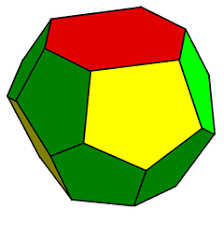
\includegraphics[]{polyhedron.png} 
\end{center} 
\newpage 

\tableofcontents

\newpage

You may be familiar with the idea of optimization as it was presented in your introductory calculus course. Given some function, we want to find the point(s) at which it is  maximized or minimized; we may refer to these points as \textbf{optimal}.\footnote{You may also be familiar with the distinction between global and local maxima/minima. In the linear programming setting, any local optimum is also a global optimum, but this does not always hold, particularly when dealing with nonlinear or nonconvex functions/constraints.} Given a function such as $f(x) = -x^2$, we know that we find its global maximum by finding the point where the derivative vanishes. 

\medskip But what if we were to impose some \textbf{constraints} on the optimal solution? For instance, what if I wanted to maximize $f(x) = -x^2$, but I also wanted the solution $x$ to satisfy the inequality $x \geq 2$? What if I also require solution to satisfy $x \leq 10$? Our old solution $x = 0$ no longer works because it fails to satisfy these constraints! 

\medskip We quickly see that these elementary methods for optimization are not enough, because they have no way of accounting for these restrictions. Problems concerned with maximizing some linear function with respect to a set of linear constraints on the solution are referred to \textbf{linear programming} problems and are the treatment of this short introduction.

\section{Examples of linear programs}

Linear programming problems are very much practical problems. In fact, optimization problems that are unconstrained are rather rare in practice. For instance, if we're a chocolate manufacturer and we're trying to finding the optimal quantity $x^*$ of chocolate bars to sell, we must at least have the constraint that $x^* \geq 0$ since we certainly can't sell a negative quantity! 

\medskip
Before providing a formalization of the form of linear programming problems, we'll take a look at some examples to build intuition.

\subsection{Alex's Apples}

Alex is an apple grower. He grows red apples, green apples, and yellow apples. He sells the red apples for $c_r$ dollars, green ones for $c_g$ dollars, and yellow ones for $c_y$ dollars. Let $x_r$, $x_g$, and $x_y$ reflect the quantities of the respective apples that Alex sells. Then Alex's total revenues are described by the function 

\[ f(x_r, x_g, x_y) = c_r x_r + c_g x_g + c_y x_y \]
 which he would like to maximize.

\medskip However, Alex can only grow so many apples because he has only $a_r$ seeds for red apples, $a_g$ seeds for green ones, and $a_y$ seeds for yellow ones. Of course, Alex cannot sell a negative quantity of apples either. The constraints on Alex's apple production are thus

\[ x_r \leq a_r \]
\[ x_g \leq a_g \]
\[ x_y \leq a_y \]
\[ x_r, x_g, x_y \geq 0 \]

This is an example of a problem that is \textbf{feasible} and bounded; that is, the set of solutions to the problem is nonempty and the optimal revenue $f(x_r^*, x_g^*, x_y^*)$ is finite.

\subsection{Xela's Xylophones}

Xela sells xylophones. She sells plastic xylophones and rosewood xylophones for $c_p$ and $c_w$ dollars respectively. Using the similar notation as the prior problem, Xela's revenues are described by the function

\[ f(x_p, x_w) = c_p x_p + c_w x_w \]

\medskip For every xylophone she produces, Xela must use $a_b$ units of base materials (think nails, screws, etc). Additionally, plastic xylophones require $a_p$ units of plastic, and rosewood xylophones require $a_w$ units of rosewood. The constraints are thus

\[ x_p + x_w \leq a_b \]
\[ x_p \leq a_p \]
\[ x_w \leq a_w \]
\[ x_w, x_p \geq 0 \]

But in addition, because rent is due, Xela wants to sell at least $\mu$ rosewood xylophones, where $\mu > a_b$. Then, with this additional constraint 
\[ x_p + x_w \geq \mu \geq a_b + 1 \] the problem becomes \textbf{infeasible} as there is no solution that can satsify this constraint and the first one.

\subsection{On notation}

The example linear programs we studied described the \textbf{objective function}\footnote{That is, the function we're trying to maximize. If we're specifically trying to minimize a function, we coud also refer to it as a \textbf{cost function}.} and constraints in terms of a system of equations and inequalities. As you may have learned, any such system can be equivalently expressed in terms of matrices. For instance, with the "Alex's Apples" program, we may let 
$$\bold{c} = \begin{bmatrix}c_r \\ c_g \\ c_y \end{bmatrix}$$ 
$$\bold{x} = \begin{bmatrix}x_r \\ x_g \\ x_y \end{bmatrix}$$ 
$$\bold{b} = \begin{bmatrix}a_r \\ a_g \\ a_y \end{bmatrix}$$ and 
$$A = \begin{bmatrix}1 & 0 & 0 \\ 0 & 1 & 0 \\ 0 & 0 & 1 \end{bmatrix}$$

Then the problem may be equivalently expressed as maximizing the function 

\[ \bold{c}^T\bold{x} \]

with respect to the constraint

\[ A\bold{x} \leq \bold{b} \]
\[ \bold{x} \geq 0 \]

It would be a good exercise to convince yourself that this is an equivalent problem. The key idea is that we can express a linear programming problem in a variety of ways, whether that be in terms of systems of equations or matrices. So we may choose which ever representation is most convenient. When discussing algorithms for solving linear programming problems, many prefer to use the matrix form since it's not only more compact but also more convenient for implementing these algorithms in code. 

\section{Defining linear programs}

Before going any further, we formally define the general linear programming problem.

\bigskip
\begin{ybox}
    \begin{definition}{(Linear program)}
        \hskip
        \medskip
        
        A linear program features a linear\footnote{a linear function is synomonous with a linear transformation here; informally, it is a function mapping its inputs to some linear combination of those inputs.} \textbf{cost function} $\bold{c}^T\bold{x}$, where $\bold{c}$ is some $n$-dimensional \textbf{cost vector} and $\bold{x}$ is a $n$-dimensional vector of decision variables. It also features a set $S$ of $m$ linear equality and inequality constraints, where the $i$th constraint is of either of the forms 

        \[ \bold{a}_i\bold{x} \leq b_i \]
        \[ \bold{a}_i\bold{x} = b_i \]
        \[ \bold{a}_i\bold{x} \geq b_i \]
        
        for some $n$-dimensional vector $\bold{a}_i$ and scalar $b_i$. We consider the problem of minimizing $\bold{c}^T \bold{x}$ subject to every constraint in $S$. A solution $\bold{x}$ satisfying all the constraints in $S$ is called \textbf{feasible}. The set of all feasible solutions is called the \textbf{feasible set}. An optimal feasible solution $\bold{x}^*$ is one that which minimizes the objective function such that $\bold{c}^T\bold{x^*} \leq \bold{c}^T\bold{y}$ for all feasible solutions $\bold{y}$. The value $\bold{c}^T\bold{x}^*$ is called the \textbf{optimal cost}.
    \end{definition}
\end{ybox}

\bigskip
For now, we're assuming that cost function, constraints, and vectors are all real-valued, but a linear program could also be integer-valued, for example. Note that any problem of maximizing a linear function $\bold{c}^T \bold{x}$ can be expressed as minimizing $-\bold{c}^T \bold{x}$, so this definition accounts for either case. It is also not too important whether or not the constraints are strict (why?)

\medskip
A linear program may not have an optimal feasible solution. However, it need not be the case that the program has no feasible solutions (although this is a possibility). Instead, it could be the case that the feasible set is unbounded and that for any supposedly optimal solution $\bold{x}^*$ and optimal cost $\bold{c}^T\bold{x}^*$, there always exists some other solution $\bold{y}^*$ such that $\bold{c}^T\bold{y}^* < \bold{c}^T\bold{x}^*$. The optimal cost in this scenario is this scenario is $-\infty$.

\subsection{Standard form linear programming problems}

\medskip
In the literature, linear programming problems are usually presented in the \textbf{standard form}. The basic idea of it is that most of the constraints is expressed as an equality, with the additional constraint that every solution $\bold{x}$ has nonnegative components. 

\bigskip
\begin{ybox}
    \begin{definition}{(Standard form linear program)}
        \hskip
        \medskip
        
        A standard form linear program is of the form
        
        \[ \text{minimize  } \bold{c}^T\bold{x} \]
        \[ \text{subject to  } \begin{cases} A\bold{x} = \bold{b} \\ 
                                             \bold{x} \geq 0 
                               \end{cases} \]
        
        where $A$ is some $m \times n$ matrix and $\bold{b}$ a $m$-dimensional vector representing the constraints.
    \end{definition}
\end{ybox}

\bigskip
It can be shown that any linear programming problem can be reduced into the standard form. We do not provide a formal proof of this, but the intuition goes as follows: for any constraint that is linear inequality like $\bold{a}_i\bold{x} \leq b_i$, we can add or subtract a \textbf{slack variable} $s_j$ such that the constraint becomes an equation like $\bold{a}_i\bold{x} + s_j = b_i$, also introducing the positivity constraint $s_j \geq 0$. Note that $s_j$ is added to the set of decision variables. If the sign of some decision variable $x_j$ is unconstrained\footnote{Some literature refers to such variables as \textbf{free}. Variables whose signs are restricted are unsurprisingly said to be \textbf{restricted}.}, we can replace it with the expression $x_j' - x_j''$, where $x_j'$ and $x_j''$ are two new decision variables subject to the positivity constraints $x_j', x_j'' \geq 0$. This follows the fact that any real number can be expressed as the difference of two nonnegative real numbers.

\bigskip
\begin{gbox}
    \begin{theorem}{(Standard form reduction)}
        Any linear program $P$ can be reduced to a linear program $P'$ in standard form via the elimination of inequalities using slack variables and the elimination of unconstrained variables. Any feasible solution $x$ to $P$ with cost vector $\bold{c}$ can be used to derive a feasible solution $x'$ to $P'$ with the same cost $\bold{c}^T\bold{x}$.
    \end{theorem}
\end{gbox}

\bigskip
The standard form is primarily adopted for the sake of constructing algorithms that solve linear programs, since expressing the constraints as equations is better suited for implementing said algorithms.

\subsection{Geometric intuition}

The algebraic presentation of the linear programming problem can be rather dense, which is why studying the geometric interpretation of these problems can be helpful for building intuition. Our study of the geometry of linear programs will be biased towards the case where the feasible set is two-dimensional, but the intuition applies for feasible sets of higher dimensions without any major hiccups.

\medskip
Let us consider the linear program 

        \[ \text{minimize  } \bold{c}^T\bold{x} \]
        \[ \text{subject to  } A\bold{x} \leq \bold{b} \]
                               
where 

        \[ A = \begin{bmatrix}1 & 0 \\ 0 & 1 \\ 1 & 0 \\ 0 & 1 \end{bmatrix}\]
        \[ \bold{b} = \begin{bmatrix}5 \\ 5 \\ 0 \\ 0\end{bmatrix}\]
        \[ \bold{c} = \begin{bmatrix}2 \\ 3\end{bmatrix} \]
        \[ \bold{x} \in \mathbb{R}^2 \]

\medskip
Equivalently, we're interested in minimizing the function 

        \[ f(x, y) = 2x + 3y \]
        
with the constraint $0 \leq x$, $x \leq 5$, $0 \leq y$, and $y \leq 5$. If we plot these inequalities on a graph and shade the regions, we get Figure 1.

\begin{figure}
    \centering
    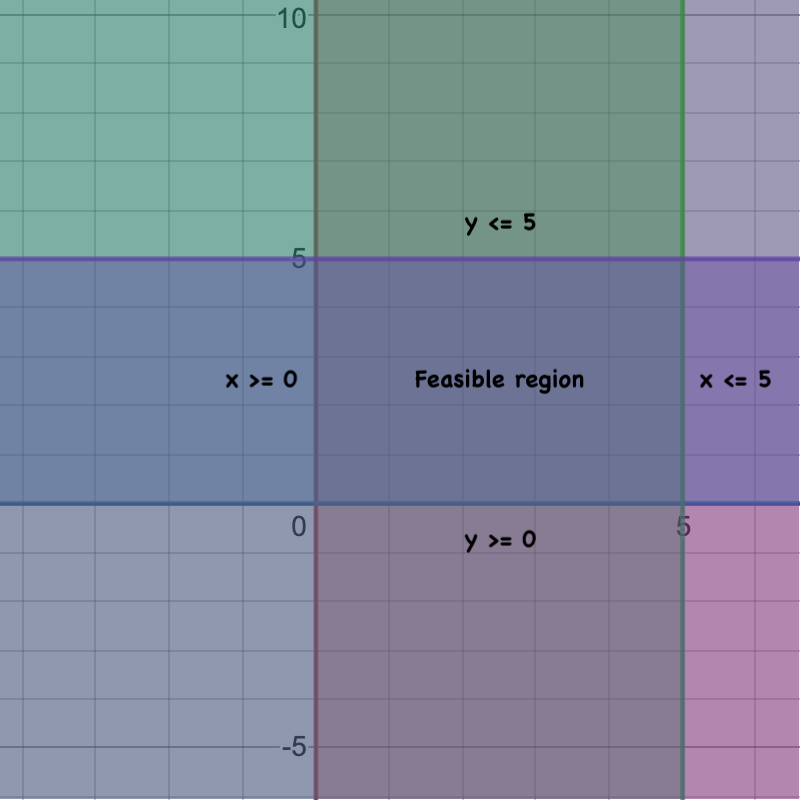
\includegraphics[scale=0.4]{figure 1.png}
    \caption{The constraints $0 \leq x_1$, $x_1 \leq 5$, $0 \leq x_2$, and $x_2 \leq 5$ as plotted on a graph. The intersection of all the colored regions is the set of feasible solutions.}
    \label{fig:my_label}
\end{figure}

\medskip
The intersection of all the inequalities' respective regions is called the \textbf{feasible region}. The lines $y = 5$, $y = 0$, $x = 5$, $x = 0$ bound the feasible region. The linear programming can now be thought of asking: \textit{which point $(x, y)$ in the feasible region will minimize the expression $2x + 3y$?}

\medskip
It turns that this optimal solution in this case is $(0, 0)$, which is a "corner" of our feasible region. This hints at a more general result, which for any linear program that which is feasible and has an optimal solution, then there exists an optimal solution that is a "corner" (alternatively, an extreme point) of the feasible region. This follows a theorem stating that every (basic) feasible solution to a linear program is a corner point of the corresponding feasible region\footnote{When discussing the geometry of linear programs, these feasible regions are better known as \textbf{polyhedra}, an example of which accompanies the title page}.

\medskip
Now imagine we did not have the constraint $x >= 0$, as in Figure 2. This illustrates the case where the feasible region is not bounded and in particular the case where there exists no optimal solution. To see this, notice that $(0, 0)$ can't be an optimal solution, since the cost for the solution $(-1, 0)$ is lower ($-2 < 0$). But $(-1, 0)$ cannot be optimal either, since the cost for $(-2, 0)$ is even lower. This chain of reasoning leads us to see that there exists no optimal solution and that the optimal cost is $-\infty$.

\begin{figure}
    \centering
    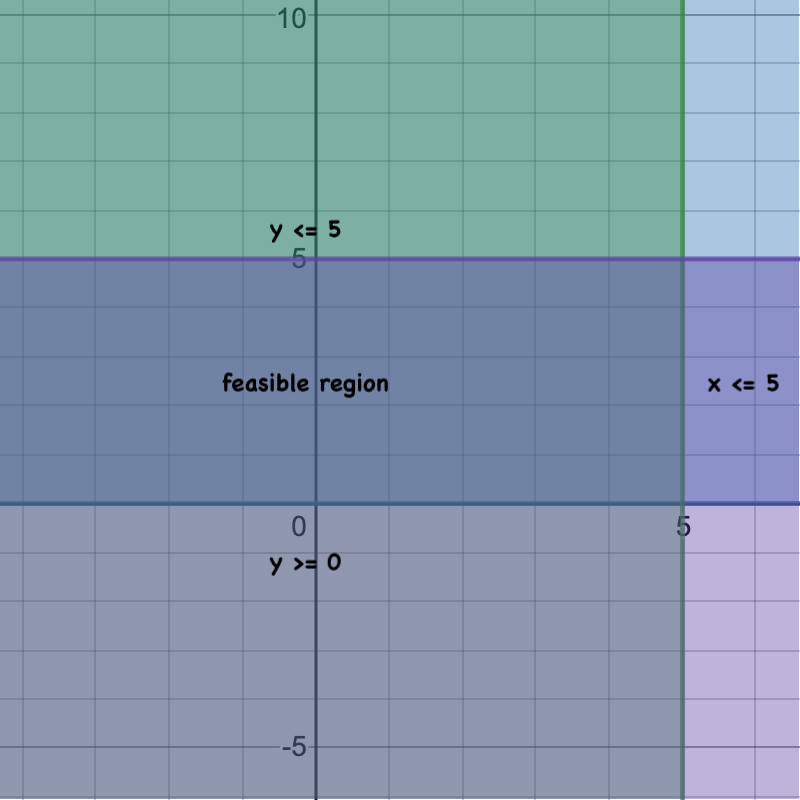
\includegraphics[scale=0.4]{figure 2.png}
    \caption{The constraints $x \leq 5$, $0 \leq y$, and $y \leq 5$ as plotted on a graph.}
    \label{fig:my_label}
\end{figure}

\section{Finding optimal solutions to linear programs}

So far, much of our discussion has centered on shaping and motivating the linear programming problem. We now turn towards discussing how to find optimal solutions to linear programs. 

\medskip
When there do not exist convenient closed forms for finding optimal solutions to any optimization problem, we typically turn towards iterative algorithms that help us move from one feasible solution towards another feasible solution that has \textit{lower} cost. This is the essence of the \textbf{simplex} method: starting with some initial feasible solution to a linear program, we move along the boundary of the feasible set towards a cost-reducing direction. After doing this enough times, we will find an optimal solution. 

\subsection{Basic solutions, basis matrices, and feasible directions}

Detailing the simplex method requires us to establish some ideas about solutions to linear programs. That is because the simplex method requires the initial feasible solution to have certain properties that are useful towards finding feasible solutions with a lower cost.

\bigskip
\begin{ybox}
    \begin{definition}{(Basic solution)}
        Consider some solution $\bold{x} \in \mathbb{R}^n$ to a linear program $P$. $\bold{x}$ is said to be a \textbf{basic solution} if and only if $\bold{x}$ satisfies all the equality constraints of $P$ and out of all the constraints satisfied by $\bold{x}$, exactly $n$ of those constraints are linearly independent\footnote{If it satisfies more than $n$ constraints, then the solution is said to be degenerate. We will not consider degeneracy here, since degenerate solutions complicate the optimization problem. However, it's worth knowing that the simplex algorithm can deal with degeneracy when augmented with certain rules.}; that is, their corresponding vectors $a_i$ are linearly independent.
        
        \medskip
        A basic solution that also happens to satisfies all the constraints of $P$ is known as a \textbf{basic feasible solution}.
    \end{definition}
\end{ybox}

\bigskip
For a geometric interpretation, the aforementioned extreme points of the feasible region constitute the basic feasible solutions. With this notion of basic solutions, we can also define basic variables and the basis matrix with the following theorem.

\bigskip
\begin{gbox}
    \begin{lemma}{(Basicity)}
        Consider the standard form linear program $P$ with constraints $A\bold{x}=\bold{b}$ and $\bold{x} \geq 0$, where $A$ is an $m \times n$ matrix\footnote{It must be the case $m \leq n$; otherwise, the program fails to have a solution, i.e. it is \textbf{infeasible}.}. Let $\bold{x}^* \in \mathbb{R}^n$ be some solution for $P$. Then $\bold{x}^*$ is a basic solution if and only if there exists a set of indices $I$ such that for $i \in I$ the columns $A_i$ are linearly independent and for all $j \in [n]$ where $j \not \in I$ we have that $x^*_j = 0$. 
    \end{lemma}
    \begin{definition}{(Basic variables and basis matrix)}
        The decision variables $x^_i$ for $i \in I$ are known as \textbf{basic variables}, every other decision variable $x_j$ is \textbf{nonbasic}. The $m \times m$ matrix
        
        \[ B = \begin{bmatrix}A_1 \dots A_{\max{(I)}}\end{bmatrix} \]
        
        is a \textbf{basis matrix}.
    \end{definition}
\end{gbox}

\bigskip
Assuming that we know what the basic variables are, this lemma enables us to find basic solutions with the system $A\bold{x} = \bold{b}$ by setting $x_i = 0 $ for $i \not \in I$ and solving for the variables $i \in I$. Where $\bold{x}_B$ indicates the vector containing the basic components of $\bold{x}$, this amounts to calculating $\bold{x}_B = B^{-1}\bold{b}$.\footnote{B is $m \times m$, and since the columns are linearly independent, its rank is $m$ and so the corresponding linear transformation is an isomorphism, which implies that $B$ is invertible.}

\medskip
The crux of the simplex algorithm is moving from one basic feasible solution $\bold{x}$ to another whilst remaining in the feasible set; geometrically, this can be interpreted choosing a vector $\bold{d}$ representing direction to move in, provided that that the resulting solution $\bold{x} + \theta \bold{d}$ for some scalar $\theta$ is still in the feasible region. This vector $\bold{d}$ is in some respect core of the simplex algorithm, so it warrants its own definition.

\bigskip
\begin{ybox}
    \begin{definition}{(Feasible direction)}
        Let $\bold{x}$ be any feasible solution. A vector $\bold{d} \in \mathbb{R}^n$ is said to be a feasible direction for $\bold{x}$ if there exists positive $\theta \in \mathbb{R}$ such that the vector $\bold{x} + \theta\bold{d}$ is feasible.
        
        \medskip
        Let $j$ be the index of some nonbasic variable $x_j$ for the constraints $A\bold{x} = \bold{b}$ and $\bold{x} \geq 0$. Then the $j$th basic direction is defined as the $n$-dimensional feasible direction $\bold{d}$ where the $i$th component $d_i = -(BA_j)_i$ for basic variables, $d_j = 1$, and $0$ otherwise (for all other nonbasic variables).
    \end{definition}
\end{ybox}

\bigskip
Why the interest in basic directions? Well, as stated in the prior section, an optimal solutions to a linear program under usual conditions will end up being one of the extreme points of the feasible region. The motivation for (feasible) basic directions is that they're always parallel to the edges of the feasible region.\footnote{Basic directions are always feasible when the solution $\bold{x}$ is not degenerate.} So, if $\bold{x}$ is some extreme point on the feasible region (i.e. it's on one of the corners), if we can move in some feasible basic direction towards another extreme point, and if the move would be cost-reducing, then we should take the move since doing so will take us closer to the optimal solution.

\medskip
Given any feasible basic direction $\bold{d}$ at a basic feasible solution $\bold{x}$, we're interested in finding how out much the cost reduces as we move towards that direction $\bold{d}$ from $\bold{x}$. This gives rise to one last definition quantifying the "rate" of change in the cost of a variable as we move in some basic direction:

\bigskip
\begin{ybox}
    \begin{definition}{(Reduced cost)}
        Given a cost vector $\bold{c}$ and basis matrix $B$ for some feasible solution $x_j$, the \textbf{reduced cost} $\bold{c}'_j$ of the decision variable of $x_j$ is \[ \bold{c}_j' = \bold{c}_j - \bold{c}_{B}^TB^{-1}A_j = \bold{c}_j - \bold{c}_{B}^T\bold{d}_j \] where $\bold{d}_j$ denotes the $j$th basic direction. The reduced cost for basic variables is $0$.
    \end{definition}
\end{ybox}

\bigskip
If the reduced cost for the $j$th variable is positive, then moving in the $j$th basic direction from some basic feasible solution will increase the cost. If it's negative, then moving in that direction will decrease the cost, which approaches what we want.

\medskip
Synthesizing everything we've discussed so far, if we wanted to find the optimal solution for some linear program, then we should start with some basic feasible solution. We can then calculate all the reduced costs $\bold{c}'$ and for some nonbasic variable $\bold{x}_j$ such that $\bold{c}_j' < 0$, we move in its respective (basic) direction $\bold{d}$ towards an adjacent basic feasible solution. The basic feasible solution $\bold{x} + \theta\bold{d}$ that we move to will have a lower cost. Figure 3 offers a visual summary of this process.

\begin{figure}
    \centering
    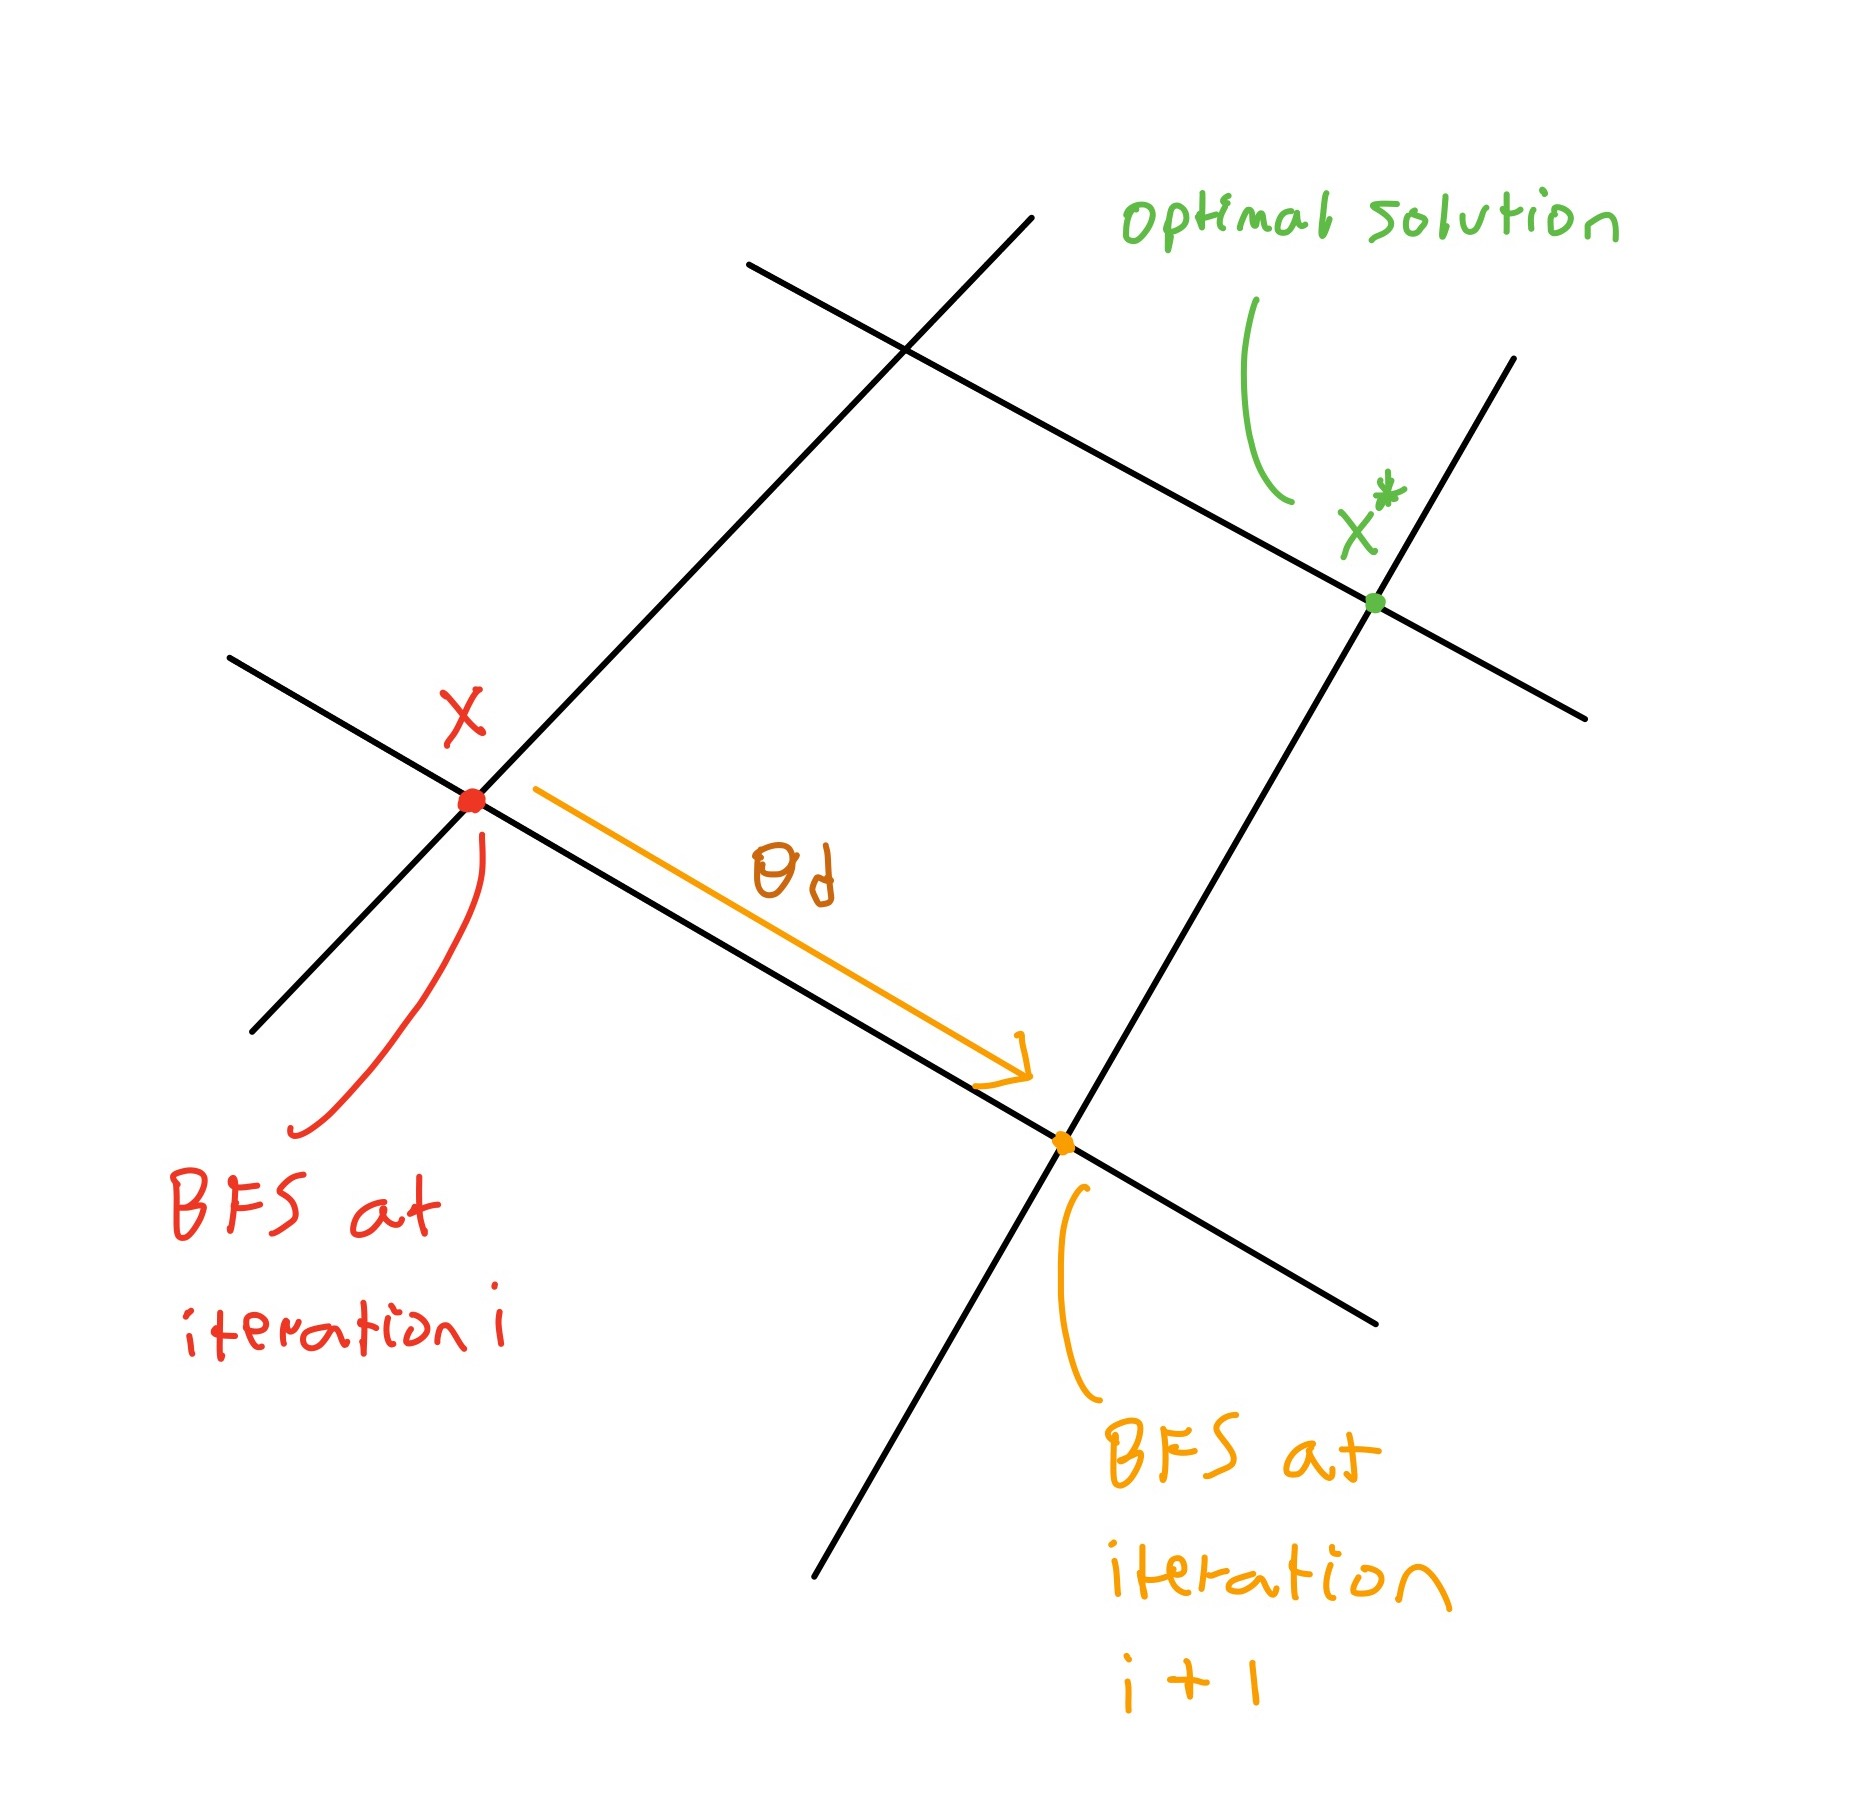
\includegraphics[scale=0.1]{figure 3.jpg}
    \caption{Starting at an initial basic feasible solution (bfs) of $\bold{x}$, if we identify $\bold{d}$ as a basic feasible direction corresponding to some nonbasic variable $x_j$, then there exists some scalar $\theta$ such that $\bold{x} + \theta \bold{d}$ is an adjacent basic feasible solution. If the reduced cost for $x_j$ is negative, this solution $\bold{x} + \theta \bold{d}$ will bear a lower cost. By applying this process again starting with $\bold{x} + \theta \bold{d}$, we will eventually reach the optimal solution $\bold{x}^*$.}
    \label{fig:my_label}
\end{figure}

\medskip
Ignoring some details such as the choice of $j$ or $\theta$, the simplex algorithm just iterates this process on each basic feasible solution obtained until the reduced cost for every variable is nonnegative, in which case the solution will be optimal\footnote{This conclusion only holds because the aforementioned phenomenon where in linear programs local minima of the cost function are also global minima. Indeed, if you've worked with a nonlinear optimization technique like gradient descent, you'll be familiar with how these techniques can sometimes get "stuck" in local minima. So be thankful for linearity!}.

\subsection{The simplex algorithm}

We finally present a simplified version of the simplex algorithm, but given our discussion above you'll find most of its steps are intuitive. 

\bigskip
\begin{bbox}
    \textbf{Simplex method}
    \medskip
    
    Let $\bold{x}^0 \in \mathbb{R}^n$ be any initial basic feasible solution for some standard form linear program $P$ with cost vector $\bold{c}$ and the constraints $A\bold{x} = \bold{b}$ and $\bold{x} \geq 0$. Let $I$ is the index set of the basic variables and where $\Bar{I}$ is the index set for the nonbasic variables. If $P$ is feasible and has no degenerate solutions and if there exists an optimal solution for $P$, then an optimal solution may be found with the following algorithm.
    
    \medskip
    \begin{algorithm}[H]
        \SetAlgoLined
        1. If it's the first iteration, assign $\bold{x} \leftarrow \bold{x}^0$.
        
        2. For $i \in \bar{I}$, compute the reduced costs $\bold{c}'_i$. If they're all nonnegative, terminate with $\bold{x}$ as an optimal solution. Otherwise, choose any $j$ such that $\bold{c}'_j < 0$.
        
        3. Let $\bold{d} = B^{-1}A_j$ (the feasible direction for the $j$th variable)\footnote{If we did not make the assumption that $P$ had an optimal solution, then we might've run into the problem that no component of $\bold{d}$ was positive, in which case the optimal cost is $-\infty$}, and let $k$ be the basic index minimizing $\theta^* = \frac{\bold{x}_k}{\bold{d}_k}$.
        
        4. Assign $x_j \leftarrow \theta$ and $\bold{x} \leftarrow \bold{x} + \theta^* \bold{d}$.\footnote{The choice of $\theta^*$ was such that the new solution will be basic where $x_j$ is now basic and where $x_k$ is no longer basic; more precisely, we are choosing a bfs adjacent to the current one.} Let the variable $x_j$ enter the basis, and let $x_k$ exit it. Go to step $2$.   
        
        \caption{Simplex}
    \end{algorithm}
    
    \medskip
    Because it's always moving in a cost-reducing direction, this algorithm will always converge to a solution within a finite number of iterations (on a programs with a bounded feasible set).
\end{bbox}

\bigskip
For the sake of simplicity, we've deliberately ignored several questions. In particular:

\bigskip
\begin{enumerate}
    \item The algorithm doesn't specify \textit{how} to algorithmically choose an initial basic feasible solution. That is because doing so require us to solve a separate and auxiliary linear program, which also be accomplished using the simplex method but not treated here.
    
    \item  We can ignore the caveat of not having degenerate solutions by choosing the smallest applicable index $j$ in step 2, but the proof of this is beyond the scope of this introduction.
    
    \item We assumed that the program $P$ had a solution to avoid dealing with the case where the optimal cost is $-\infty$. We could've actually detected this by checking if none of the components of the chosen basic direction were positive, in which case we can actually conclude that feasible region is unbounded and terminate (but the proof of this is also beyond our scope).
    
    \item We also didn't justify the choice for $\theta^*$ for similar reasons as above.
\end{enumerate}
 
\medskip
\subsection{Why simplex?}

In Section 2.2, we hinted that for programs that are feasible, the optimal solution, if it exists, will be a basic feasible solution. It turns out that there are finitely many basic solutions to a linear program, because there are only $n \choose m$ ways to $m$ columns from a $m \times n$ matrix $A$ to possibly form a basis matrix, and each basis matrix uniquely corresponds to a basic solution.  

\medskip
One could imagine that to find the optimal solution, we could just check every basic solution and identify the one producing the lowest cost as optimal. This certainly works, but for large enough linear programs the simplex method is on average more efficient in terms of the number of solutions it checks before finding the optimal one. The exact time complexity of the simplex method varies by the implementation\footnote{Implementing the simplex method using the same steps verbatim as the algorithm above turns out to be quite inefficient; there exists implementations using \textbf{tableaux} representations of linear programs that offers significant performance improvements}, but for a typical linear program the simplex method runs in time polynomial to $m$ and $n$ (the dimensions of the matrix $A$). For certain unusual programs, simplex indeed visits all the extreme points of the feasible region, and so its worst-case time complexity is exponential.

\medskip
For more computationally-minded readers, the supplementary materials provide a Python program implementing the simplex method in nearly one-to-one correspondence with the steps of algorithm provided above. 

\section{Further readings}
(Bertsimas and Tsitsiklis, 1997) offers a comprehensive but dense introduction to linear optimization and in particular devotes an entire chapter towards deriving the simplex method and efficient implementations of it. There are also many great resources scattered across the internet that cover LP and the simplex method with motivating intuition and examples, in particular  \href{https://mitocw.ups.edu.ec/courses/electrical-engineering-and-computer-science/6-046j-design-and-analysis-of-algorithms-spring-2015/lecture-notes/MIT6_046JS15_lec15.pdf}{this}, \href{https://www2.isye.gatech.edu/~sahmed/isye3133b/simplex}{this}, and \href{https://ocw.mit.edu/courses/electrical-engineering-and-computer-science/6-251j-introduction-to-mathematical-programming-fall-2009/lecture-notes/MIT6_251JF09_lec05.pdf}{this}. 

\end{document}

